\scanpage{59}
% L01-03, upper groupoid notes
$\unsure{C|\mathcal{C}|\mathscr{C}}$ groupoïde.
$G\inserted{\subset\mathrm{Aut}(C)}$ transitif sur $C_0=\mathrm{Ob}\,C$\quad $e\in C_0$\quad $H=G_e$

$\Gamma$ normalisateur de $G$.
$\Gamma^{\unsure{0|\circ}}$ centralisateur de $\unsure{G|C}$.
\[C_0\simeq G/H\]
% L04
\diagram{\begin{tikzcd}[ampersand replacement=\&]
1\arrow[r]\&\Gamma^0\arrow[r]\&\Gamma\arrow[r]\&\mathrm{Aut}(G)
\end{tikzcd}}
% L05-06
$e\in\mathrm{Ob}\,C=C_0$

$\gamma_{C_0}$ connu quand on \unsure{connaît|connait} $\gamma.e$
% L07-08
\diagram{\begin{tikzcd}[ampersand replacement=\&]
1\arrow[r,no head]\&\Gamma^{\deleted{\unsure{2|1}}\unsure{1|2}}\arrow[r,no head]\arrow[d,no head,"\unsure{f}"']\arrow[dr]\&\Gamma^0\arrow[r]\&N(H)/H\\
\&\unsure{H}\&\mathrm{Aut}_H(\pi_e)
\end{tikzcd}}
\figure{\begin{tikzpicture}
\draw (0,0) .. controls (.12,1) and (.35,1.7) .. (.6,2.2);
\draw[->,very thick] (0,0)--(2,1.25) node[midway,above] {$f$};
\fill (0,0) circle (2pt) (.6,2.2) circle (2pt) (2,1.25) circle (2pt);
\node[below] at (0,0) {$e$};
\draw (3.6,.1) .. controls (4.4,1) and (5.3,1.3) .. (6.1,1.6);
\fill (3.6,.1) circle (1.8pt); \node[below] at (3.6,.1) {$\gamma e$};
\end{tikzpicture}}
\par\noindent\rule{\linewidth}{.4pt}

% L09-11, graph notes
$K=K_0,K_1,\ K_1\longrightarrow K_0\ \unsure{\mathrm{inv}}$ (graphe \inserted{connexe}), $G$ grp, \deleted{d'automorphismes de} \inserted{opérant sur} $K$ on suppose que $G$ est transitif sur l'ens $K_1$ des arcs de $K$
% L12-13
\diagram{\begin{tikzcd}[ampersand replacement=\&]
K_1\simeq G/\unsure{H|\mathbb{H}}_1\arrow[d]\\
K_0=G/H_0
\end{tikzcd}}
\[\sigma\in N(H)/H\qquad\sigma^2=1\]

% L14
$C\inserted{=(C_0,C_1)}$ groupoïde, $\deleted{\unsure{C}}$ $G$ opère sur $C_0$
% L15
\diagram{\begin{tikzcd}[ampersand replacement=\&]
\unsure{K_\alpha|K}\arrow[r,hook]\&C
\end{tikzcd}}
$G$-morphisme on suppose
\diagram{\begin{tikzcd}[ampersand replacement=\&]
K_0\arrow[r,"{\deleted{\unsure{\mathrm{équi}}}\ \sim}"]\&C_0
\end{tikzcd}}

% L16, small arrows at left
\figure{\begin{tikzpicture}
\fill (0,0) circle (2pt); \node[below left] at (0,0) {$e$};
\draw[->,very thick] (0,0)--(1.8,.8) node[right] {$e'$};
\node[below left] at (3,-.2) {$\gamma e$};
\draw[->,thick] (3,-.2)--(4.8,.6) node[right] {$\gamma e'$};
\end{tikzpicture}}
% L16-18, lower chains
\diagram{\begin{tikzcd}[ampersand replacement=\&]
1\arrow[r]\&\Gamma^0\arrow[r]\&\Gamma\arrow[r]\&\mathrm{Aut}_*(G)
\end{tikzcd}}
\diagram{\begin{tikzcd}[ampersand replacement=\&]
\Gamma\arrow[r,"\unsure{/}" description]\&G
\end{tikzcd}}
\diagram{\begin{tikzcd}[ampersand replacement=\&]
1\arrow[r]\&\Gamma^1\arrow[r]\&\Gamma^0\arrow[r]\&\deleted{G_*}\arrow[r]\&N(H_0)/H_0
\end{tikzcd}}
\diagram{\begin{tikzcd}[ampersand replacement=\&]
\deleted{1}\arrow[r,no head,"\deleted{\longrightarrow}" description]\&
\deleted{\Gamma^2}\arrow[r,no head,"\deleted{\longrightarrow}" description]\&
\Gamma''\arrow[r,hook]\&\mathrm{Aut}_G\pi_e
\end{tikzcd}}
% L19-20, bottom drawing and notations
\figure{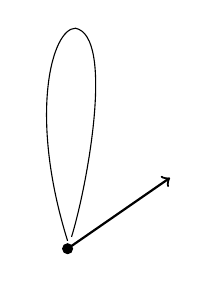
\begin{tikzpicture}
\fill (0,0) circle (2pt);
\draw (0,.1) .. controls (-.5,1.7) and (-.2,2.8) .. (.1,2.8)
 .. controls (.6,2.7) and (.25,.8) .. (.05,.15);
\draw[->,thick] (0,0)--(1.3,.9);
\end{tikzpicture}}
\[
\pi_e,\ \deleted{\unsure{K_e|\Pi_e}}\qquad
\begin{gathered}\mathrm{Hom}(e,e')\\\Vert\\\Pi_{e,e'}\end{gathered}
\qquad\Pi_e\qquad *
\]
\[\unsure{\mathrm{Aff}_{H_0}(\pi_e)|N_{H_0}(\pi_e)}\]
% archive sheet number: 58
